\documentclass[11pt]{article}

\usepackage{amsmath}
\usepackage{amsfonts}
\usepackage{amsthm}
\usepackage{blkarray}
\usepackage{caption}
\usepackage{enumitem}
\usepackage{hyperref}
\usepackage{mathtools}
\usepackage{tikz}
\usepackage[top=1.5cm,bottom=2cm,left=1.25cm,right=1.75cm,marginparwidth=1.75cm]{geometry}
\setlength{\parindent}{0cm}

\newcommand{\n}{\vspace{0.3cm}}
\newtheorem{theorem}{Theorem}

\def\lc{\left\lceil}
\def\rc{\right\rceil}
\def\lf{\left\lfloor}
\def\rf{\right\rfloor}

\newcommand{\C}{\mathbb{C}}
\newcommand{\N}{\mathbb{N}}
\newcommand{\Q}{\mathbb{Q}}
\newcommand{\R}{\mathbb{R}}
\newcommand{\Z}{\mathbb{Z}}

\title{\vspace{-1.0cm}CSCI 5304 Homework 5}
\author{Fletcher Gornick}

\begin{document}
\maketitle
\begin{enumerate}
	\item Let \(A\) be the matrix shown to the right.
			      \(A = \left( \begin{array}{rr} -2 & 2 \\ 0 & 1 \\ 1 & 0 \\ 0 & 0 \end{array} \right)\)
\begin{enumerate}
	\item What are the nonzero singular values of \(A\)? \n\\
	      To retrieve the singular values of \(A\) we must first find the eigenvalues of \(A^T A\),
	      \[A^T A =
	      \left( \begin{array}{rrrr} -2 & 0 & 1 & 0 \\ 2 & 1 & 0 & 0 \end{array} \right)
	      \left( \begin{array}{rr} -2 & 2 \\ 0 & 1 \\ 1 & 0 \\ 0 & 0 \end{array} \right)
	      = \left( \begin{array}{rr} 5 & -4 \\ -4 & 5 \end{array} \right).
	      \]
	      \(p_\lambda(A) = \det(A^T A - \lambda I) = (5 - \lambda)^2 - 16 \implies \lambda_1 = 9, \;\; \lambda_2 = 1\). \n\\
	      The nonzero singular values of \(A\) are \(\sigma_1 = \sqrt\lambda_1 = 3\), \(\sigma_2 = \sqrt\lambda_2 = 1\). \n

	\item If \(A = U \Sigma V^T\) is the SVD of \(A\), what is the matrix \(V\)?  What is \(\Sigma\)? \n\\
	      \(V\) represents the set of right-singular vectors of \(A\), which can also be thought of as the set of orthonormal eigenvectors of \(A^T A\).
	      \[A^T A v_1 = \lambda_1 v_1 \implies \begin{array}{r} 5v_{11} - 4v_{12} = 9v_{11} \\ 5v_{12} - 4 v_{11} = 9v_{12}\end{array} \implies v_1 = \binom1{-1}\]
	      \[A^T A v_2 = \lambda_1 v_2 \implies \begin{array}{r} 5v_{21} - 4v_{22} = v_{21} \\ 5v_{22} - 4 v_{21} = v_{22}\end{array} \implies v_1 = \binom11.\]
	      Now we can use Gram-Schmidt to orthonormalize \(v_1\) and \(v_2\) (easy since \(v_1\) and \(v_2\) already orthogonal):
	      \[
		      v_1 = \binom1{-1} \to
		      \left(\begin{array}{r}\tfrac{1}{\sqrt2} \\ \tfrac{-1}{\sqrt2} \end{array}\right),
		      \quad v_2 = \binom11 \to
		      \left(\begin{array}{r}\tfrac{1}{\sqrt2} \\ \tfrac{1}{\sqrt2} \end{array}\right).
	      \]
        Now we have our matrix \(V\), and \(\Sigma\) is just a \(4 \times 2\) matrix with the singular values in descending order along the upper diagonal:
        \[V = \left(\begin{array}{rr} \tfrac{1}{\sqrt2} & \tfrac{1}{\sqrt2} \\ \tfrac{-1}{\sqrt2} & \tfrac{1}{\sqrt2} \end{array}\right), \quad \Sigma = \left( \begin{array}{rr} 3 & 0 \\ 0 & 1 \\ 0 & 0 \\ 0 & 0 \end{array} \right).\]
	\item Find the first two columns of the matrix \(U\). \n\\
    The first two columns of \(U\) correspond to the left-singular vectors of \(A\), or the first two left-eigenvectors of \(AA^T\).  We already know the eigenvalues for \(AA^T\): \(\lambda_1 = 3, \lambda_2 = 1, \lambda_3 = \lambda_4 = 0\).  So we just need to find the eigenvectors corresponding to \(\lambda_1, \lambda_2\) and orthonormalize them.
    \[
    AA^T =
    \left( \begin{array}{rr} -2 & 2 \\ 0 & 1 \\ 1 & 0 \\ 0 & 0 \end{array} \right)
    \left( \begin{array}{rrrr} -2 & 0 & 1 & 0 \\ 2 & 1 & 0 & 0 \end{array} \right)
    = \left(\begin{array}{rrrr}
        8 & 2 & -2 & 0 \\ 2 & 1 & 0 & 0 \\ -2 & 0 & 1 & 0 \\ 0 & 0 & 0 & 0
        \end{array}\right).
    \]
    \[
    u_1^T AA^T = \lambda_1 u_1^T \implies
    \begin{array}{r}
        8u_{11} + 2u_{12} - 2u_{13} = 9u_{11} \\
        2u_{11} + u_{12} = 9u_{12}            \\
        u_{13} - 2u_{11} = 9u_{13}
    \end{array}
    \implies u_1 = (-4, -1, 1, 0)^T
    \]
    \[
    u_2^T AA^T = \lambda_1 u_2^T \implies
    \begin{array}{r}
        8u_{21} + 2u_{22} - 2u_{23} = u_{21} \\
        2u_{21} + u_{22} = u_{22}            \\
        u_{23} - 2u_{21} = u_{23}
    \end{array}
    \implies u_2 = (0, 1, 1, 0)^T
    \]
    Again, since these two vectors are already orthogonal, we just need to normalize them,
    \[
    u_1 = \left(\tfrac{-4}{3\sqrt2}, \tfrac{-1}{3\sqrt2}, \tfrac{1}{3\sqrt2}, 0\right)^T, \quad
    u_2 = \left(0, \tfrac{1}{\sqrt2}, \tfrac{1}{\sqrt2}, 0\right)^T.
    \]
    
	\item Find the matrix of rank 1, that is the closest to \(A\) in the 2-norm sense, i.e. the matrix \(A_1\) which minimizes \(\lVert A - B \rVert_2\) over all \(4 \times 2\) matrices \(B\) that are of rank 1. \n\\
    By the Eckart-Young theorem, we know this matrix must be:
    \[B = A_1 = \sum_{k=1}^1 \sigma_k u_k v_k^T = 3
    \left(\begin{array}{r} \tfrac{-4}{3\sqrt2} \\ \tfrac{-1}{3\sqrt2} \\ \tfrac{1}{3\sqrt2} \\ 0 \end{array}\right)
    \left(\begin{array}{rr} \tfrac{1}{\sqrt2} & \tfrac{-1}{\sqrt2} \end{array}\right) =
    \left(\begin{array}{rr} -2 & 2 \\ -1/2 & 1/2 \\ 1/2 & -1/2 \\ 0 & 0 \end{array}\right).
    \]
\end{enumerate}

	\item Consider the problem \(\min_x \lVert b - Ax \rVert_2\) in the situation where \(A\) is \(m \times n\) and \(m < n\) (`underdetermined').
	      \begin{enumerate}
		    \item Using what you've learned from the URV decomposition, find the set of \textbf{all} least-squares solutions.  Show that the least-squares solution \(x_*\) of smallest norm must belong to Ran\((A^T)\).  For the rest of the exercise assume \(A\) is of full rank. \n\\
          The solution to the least squares problem is some (not necessarily unique) vector \(x_*\) such that \(Ax_* = b_*\) where \(b_*\) is the orthogonal projection of \(b\) onto the space spanned by \(A\):
          \[b = b_* + b_\perp, \quad b_\perp \in \text{Null}(A^T), \;\; b_* \in \text{Ran}(A).\]
          Now, since \(b_\perp \in \text{Null}(A^T)\), \(A^T b = A^T(b_* + b_\perp) = A^T b_* + A^T b_\perp = A^T b_*\), meaning \(A^T Ax_* = A^T b\).  Plugging in \(A = URV^T\), we get

          \[A = URV^T = (U_1 \; U_2) \begin{pmatrix} C & 0 \\ 0 & 0 \end{pmatrix} \binom{V_1^T}{V_2^T} = U_1 C V_1^T, \quad C \in \R^{r \times r}, \; U_1 \in R^{m \times r}, \; V_1 \in \R^{n \times r}.\]
          \begin{align*}
            A^T Ax_* = A^T b &\iff V_1 C^T U_1^T U_1 C V_1^T x_* = V_1 C^T U_1^T b \\
            &\iff C V_1^T x_* = U_1^T b.
          \end{align*}

          \(CV_1^T\) is a full rank \(r \times n\) matrix (\(r < n\)), so the set of \textbf{all} solutions is the set of all \(x\) such that \(C V_1^T x = U_1^T b\).  This can be found by augmenting \(U_1^T b\) onto the matrix \(C V_1^T\) and performing row operations and backsolving for basis vectors that span the solution space. \n

          From lecture, we know that the least squares solution to \(\min_x \lVert Ax - b \rVert_2\) is \(A^\dag b + w\), where \(A^\dag\) is the pseudo-inverse of \(A\), and \(w \in \text{Null}(A)\).  So if we want the least-squares vector with minimum norm, we take \(w = 0\), and see that \(x_* = A^\dag b \in \text{Ran}(A^T)\). \n
          
		      \item Find a method for computing \(x_*\) which involves a form of normal equations.
            \[x_* = (A^T A)^{-1} A^T b.\]
		      \item Find a method for computing \(x_*\) which involves a QR factorization.
            \[x_* = R^{-1} Q^T b\]
		      \item Find a method for computing \(x_*\) based on the SVD.
            \[x_* = (\Sigma V^T)^{-1} U^T b = V \Sigma^{-1} U^T b,\]
            Where \(\Sigma^{-1}\) is just a diagonal matrix with \(\sigma_{ii} = 1 / \sigma_i\).
	      \end{enumerate}

	\item Paul, Jane, and Ann, share information about their likes and dislikes of movies in order to make decisions about selecting films to see. They rates films they see with a scale of 0 to 10, (10 means they liked the movie very much). Here is the status of their table of ratings when Ann was interested in a new film which soon came to a ’theater near her’ (titled ’Title 6’ in the table):
	      \begin{center}
		      \begin{tabular}{|c|c|c|c|c|c|c|}
			      \hline
			           & Title 1 & Title 2 & Title 3 & Title 4 & Title 5 & Title 6 \\
			      \hline
			      Paul & 4       & 9       & 2       & 7       & 8       & 3       \\
			      \hline
			      Jane & 8       & 3       & 6       & 4       & 3       & 8       \\
			      \hline
			      Ann  & 4       & 8       & 1       & 4       & 6       & ?       \\
			      \hline
		      \end{tabular}
	      \end{center}
	      \begin{enumerate}
		      \item\ [QR solution] Ann reasoned as follows: she will give the `similarity’ coefficients \(\alpha\) and \(\beta\) for Paul and Jane respectively.  If the missing rating (call it \(\delta\)) were known then the row of Ann’s ratings should be the closest in the least-squares sense to the row
		      \[\alpha * (\text{Paul's ratings}) + \beta * (\text{Jane's ratings})\]
		      Determine, \(\alpha\), \(\beta\) and the induced rating \(\delta\) for Ann for `Title 6'.  Is Ann’s taste closer to Paul’s or to Jane’s?
          \[
            A = \begin{pmatrix} 4 & 8 \\ 9 & 3 \\ 2 & 6 \\ 7 & 4 \\ 8 & 3 \end{pmatrix}
            \implies
            Q = \begin{pmatrix} 0.2734 & 0.7165 \\ 0.6152 & -0.2731 \\ 0.1367 & 0.6096 \\ 0.4785 & -0.0029 \\ 0.5469 & -0.2009 \end{pmatrix}, \;\;
            R = \begin{pmatrix} 14.6287 & 8.4081 \\ 0 & 7.9564 \end{pmatrix} \;\;\to\;\;
            x = R^{-1}Q^T b.
          \]
          By method of QR factorization, we see that \(x = (0.7704, 0.0093)^T\), so \(\alpha=0.7704\), \(\beta=0.0093\).  To approximate Ann's score, we get \(\delta = 3\alpha + 8\beta = 3 \cdot 0.7704 + 8 \cdot 0.0093 = 2.3855\). \n

		      \item\ [SVD solution] Ann reasoned as follows: Her score, say \(\delta\), for `Title 6' should be selected in such way that when added in, the rank of the resulting matrix should be the smallest possible.  Instead of rank she uses the smallest singular value: the smallest singular value of the resulting matrix should be as small as possible.  By plotting the \color{red} smallest singular value \color{black} of the filled matrix against the score \(\delta\), determine the best score. \n\\
            You can see the plot on the next page, but it looks like the rating which yields the smallest singular value is around 2.4, which agrees with our answer of 2.3855 in the previous problem.
            
            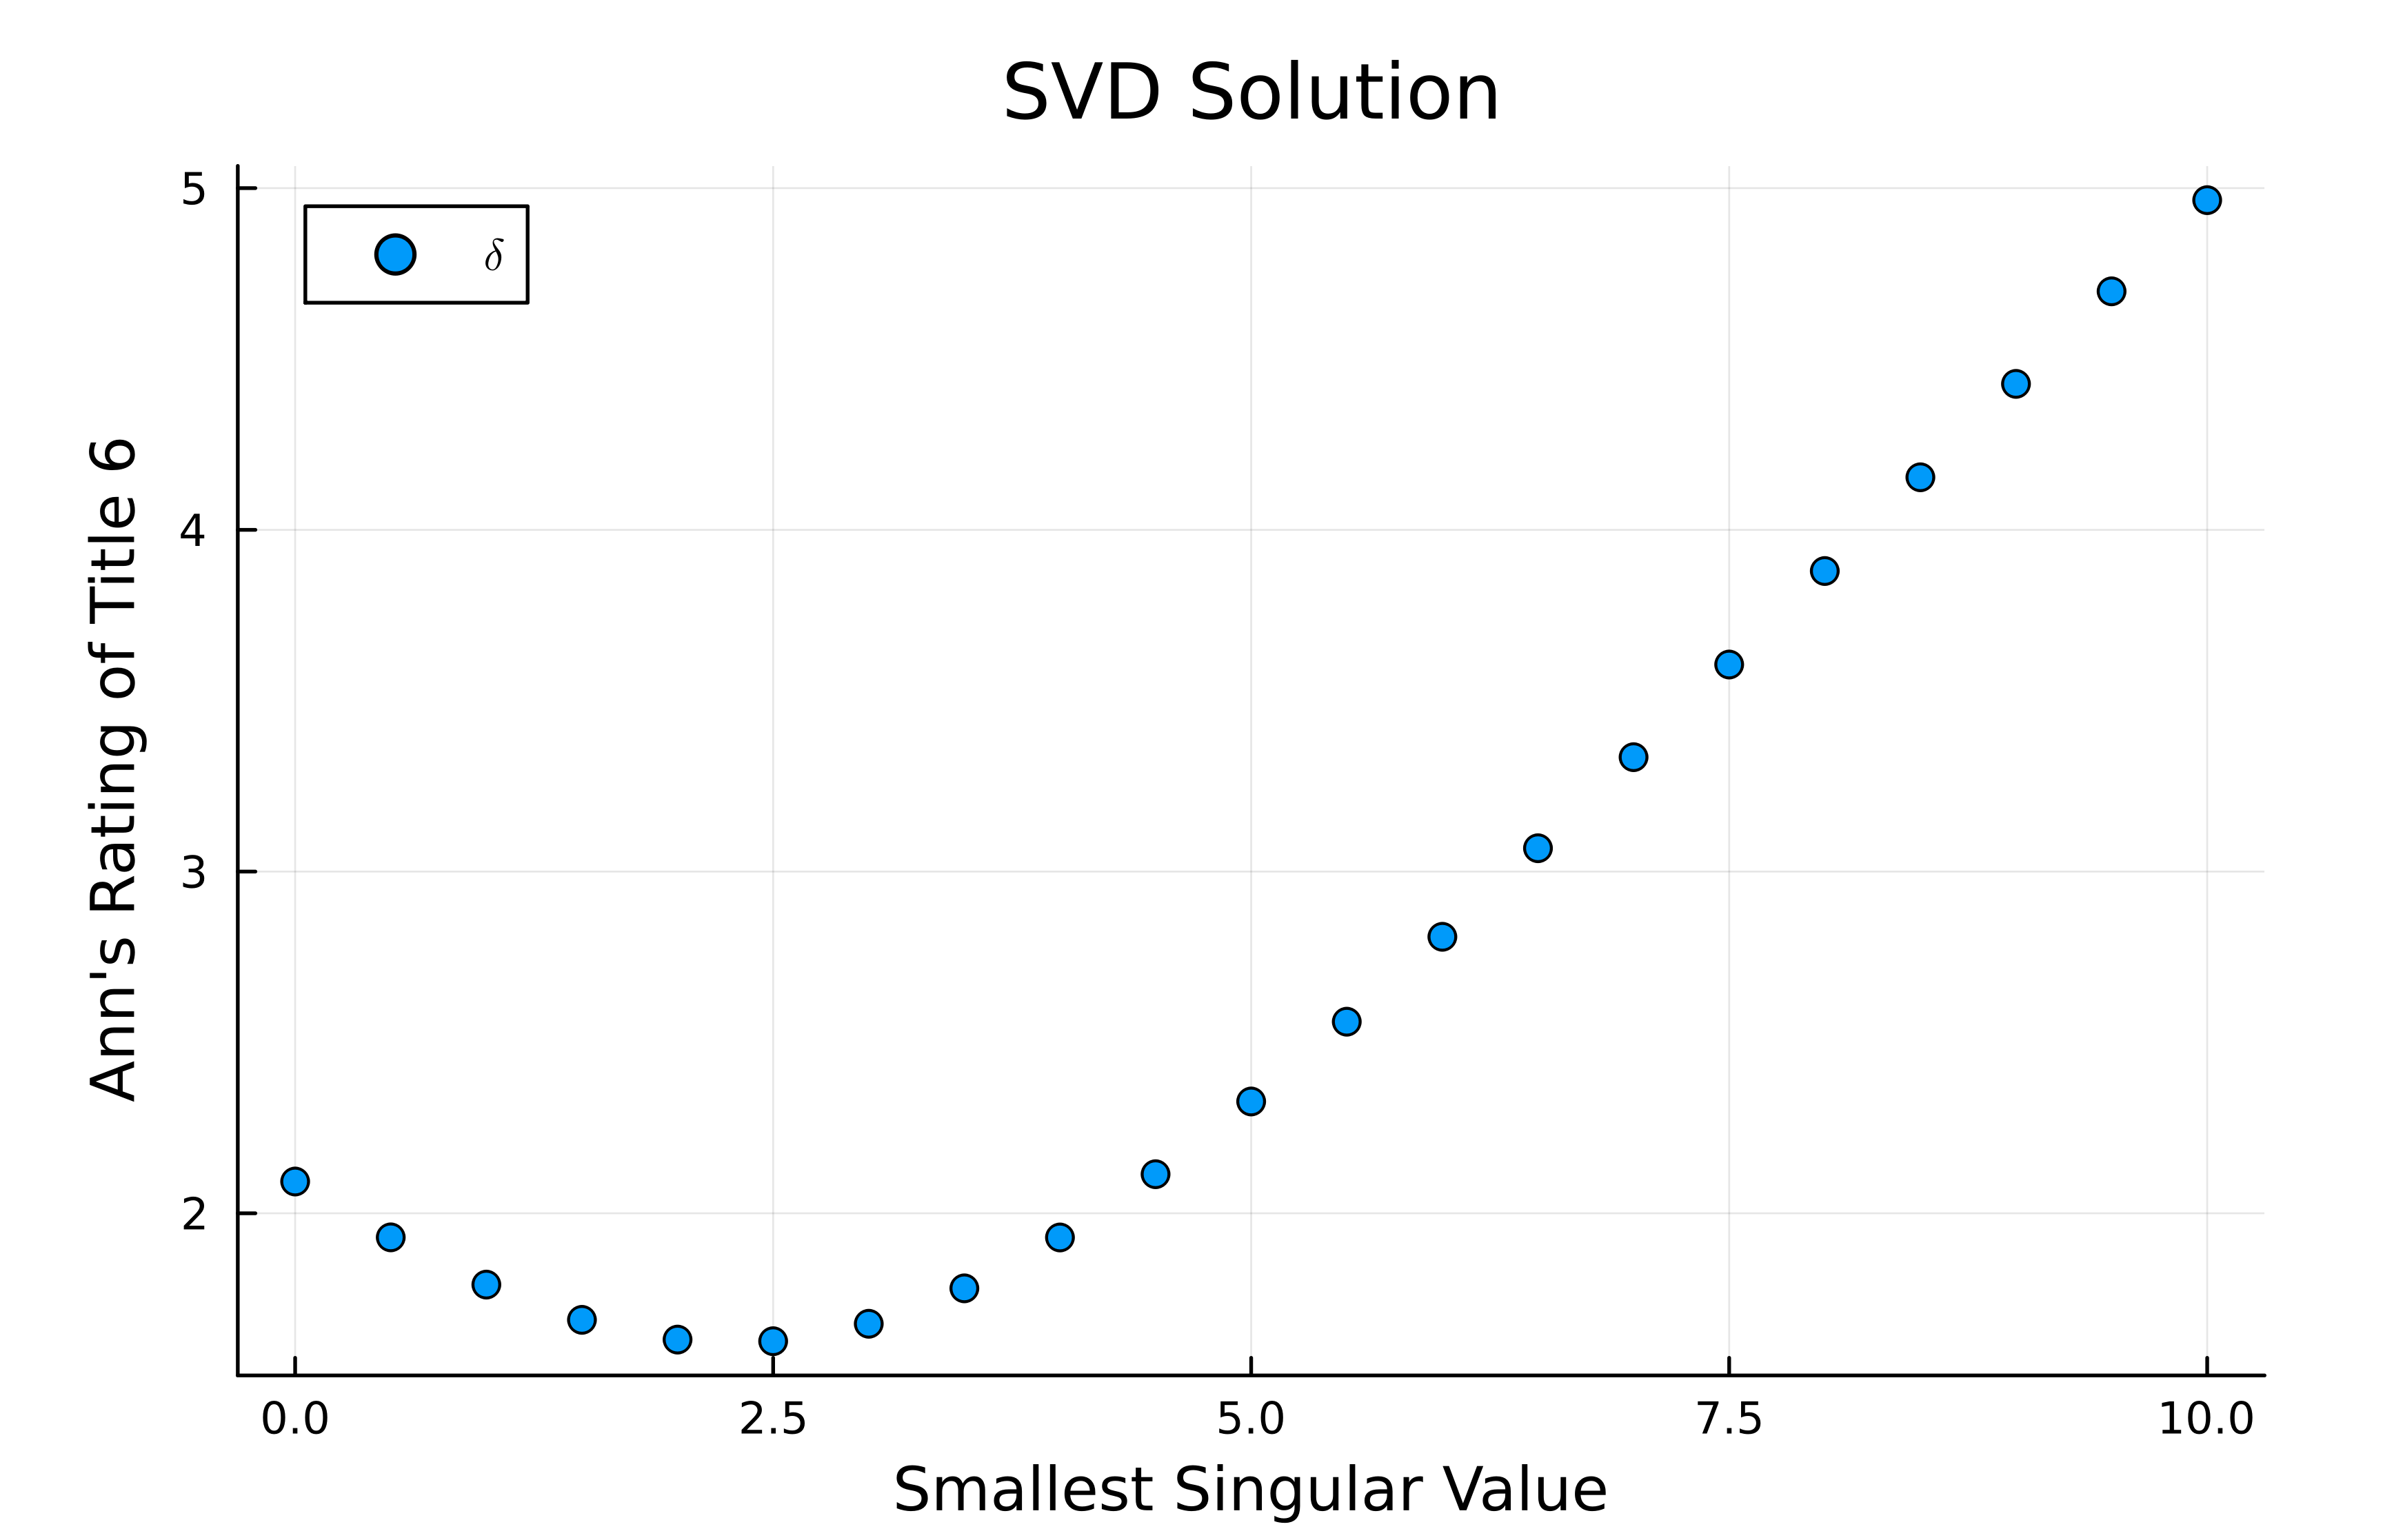
\includegraphics[width=0.8\textwidth]{plot.png}
	      \end{enumerate}

	\item For any nonzero matrix \(A\), show that
	      \begin{enumerate}
		      \item \(AA^\dag v = v\) for any \(v\) in Ran(\(A\)).
            \begin{proof}
              \(v = Aw\) for some \(w\), means that
              \[A A^\dag v = v \iff A (A^T A)^{-1} A^T A w = Aw\]
              Since \((A^T A)^{-1} A^T A = I\), we get \(AIw = Aw\) which is clearly true.
            \end{proof}
		      \item \(A^\dag x = 0\) for any \(x\) in Null(\(A^T\)).
            \begin{proof}
              \(A^T x = 0 \implies A^\dag x = (A^T A)^{-1} A^T x = (A^T A)^{-1} \cdot 0 = 0\)
            \end{proof}
		      \item \((A^T)^\dag = (A^\dag)^T\).
            \begin{proof}
              \((A^T)^\dag = ((A^T)^T (A^T))^{-1} (A^T)^T = (A A^T)^{-1} A = A^{-T}A^{-1}A = ((A^T A)^{-1} A^T)^T = (A^\dag)^T\)
            \end{proof}
		      \item \((A^\dag)^\dag = A\).
            \begin{proof} \begin{align*}
                (A^\dag)^\dag = ((A^T A)^{-1} A^T)^\dag &= (((A^T A)^{-1} A^T)^T (A^T A)^{-1} A^T)^{-1} ((A^T A)^{-1} A^T)^T \\
                &= ((A^{-1} A^{-T} A^T)^T A^{-1} A^{-T} A^T)^{-1} (A^{-1} A^{-T} A^T)^T \\
                &= (A^{-T} A^{-1})^{-1} A^{-T} \\
                &= A A^T A^{-T} = A.
              \end{align*}
            \end{proof}
	      \end{enumerate}

	\item Let \(A\) be a matrix with singular values \(\sigma_1 \geq \sigma_2 \geq \dots \geq \sigma_r > 0\), and \(E\) be a perturbation matrix such that \(\lVert E \rVert_2 < \sigma_r\).  Show that rank(\(A+E\)) \(\geq\) rank(\(A\)).
    \begin{proof}
      Let \(\text{rank}(A) = r\) and suppose (to the contrary) \(\lVert E \rVert_2 < \sigma_r\) and \(\text{rank}(A+E) = k < r\).  If \(A = U \Sigma V^T\) is the SVD of \(A\), then by the Eckart-Young theorem, \(A_k = \sum_{i=1}^k \sigma_i u_i v_i^T\) is the matrix of rank \(k\) closest to \(A\), and is distance \(\sigma_{k+1}\) away.  That is,
      \[\min_{\text{rank}(B) = k} \lVert A - B \rVert_2 = \lVert A - A_k \rVert_2 = \sigma_{k+1}.\]
      Now let's take a look at matrix \(A+E\),
      \[\lVert A - (A+E) \rVert_2 \;=\; \lVert E \rVert_2 \;<\; \sigma_r \;\leq\; \sigma_{k+1} \;=\; \lVert A - A_k \rVert_2.\]
      This clearly contradicts the Eckart-Young theorem, so we can conclude that \(\text{rank}(A+E) \geq \text{rank}(A)\).
    \end{proof}

	\item[9.] Apply Gershgorin’s theorem to find a domain where the eigenvalues of \(A\) are located for the following matrices
		\[
			A_1 = \left(\begin{array}{rrr} 1 & -1 & -1 \\ 1 & 2 & 3 \\ 2 & -4 & 1 \end{array}\right) \quad
			A_2 = \left(\begin{array}{rrr} -i & 0 & i \\ 1 & 0 & 1 \\ 0 & 1+i & i \end{array}\right) \quad
			A_3 = \left(\begin{array}{rrr} 1 & i & -i \\ -i & 2 & 0 \\ i & 0 & 3 \end{array}\right)
		\]
		The region (complex or real) you find should be the smallest possible that can be determined by using (the row version of) the Gershgorin theorem. \n\\
    Let \(D(x,r) \subseteq \C\) define a closed disc in the complex plane centered at \(x\) with radius \(r\).  We will use finite unions of these discs to describe the following eigenvalue domains.
    \[\lambda(A_1) \in D(1,6), \quad \lambda(A_2) \in D(0,2) \cup D(i,\sqrt2), \quad \lambda(A_3) \in D(1,2) \cup D(3,1).\]

	\item[10.] The matrix \(A\) shown on the right arises in boundary value problems with periodic boundary conditions.
		\begin{enumerate}
			\begin{minipage}{0.6\textwidth}
				\item What is the inertia of this matrix?
				\item What does Gershgorin’s theorem give for this matrix?
				\item This matrix is almost tridiagonal.  Is this structure preserved by the QR algorithm?
				\item Show a sequence of Givens rotations to transform this matrix into tridiagonal form (\(T = QAQ^T\) where \(Q\) is unitary, \(T\) is tri-diagonal).  What is the order of the number of operations required? Illustrate the process on a \(5 \times 5\) example (pattern only - no values).
			\end{minipage}
			\begin{minipage}{0.4\textwidth}
        \(\;\;\left(\begin{array}{rrrrrr}
        2      & -1     & 0      & \hdots & 0      & -1     \\
        -1     & 2      & -1     & \hdots & -1     & 0      \\
        0      & -1     & 2      & \hdots & 0      & -1     \\
        \vdots & \vdots & \vdots & \ddots & \vdots & \vdots \\
        -1     & 0      & -1     & \hdots & 2      & -1     \\
        0      & -1     & 0      & \hdots & -1     & 2      \\
        \end{array}\right)\)
			\end{minipage}
		\end{enumerate}

	\item[12.] Given a matrix \(X\) of size \(m \times n\) of full column rank, find the inertia of a matrix of the form
		\[B = \begin{pmatrix} D & X \\ X^T & 0 \end{pmatrix}\]
		where it is assumed that \(D\) is a diagonal matrix (of size \(m \times m\)) with positive diagonal entries.  Find the inertia when \(D\) is any nonsingular symmetric matrix (with say \(p\) positive eigenvalues and \(m-p\) negative eigenvalues) but \(X\) is an \(m \times m\) matrix (of full rank). Note: you can assume that \(D\) - is diagonal nonsingular with \(p\) positive entries on the diagonal.
\end{enumerate}
\end{document}
